\documentclass[a4paper]{article}

%% Language and font encodings
\usepackage[english]{babel}
\usepackage[utf8x]{inputenc}
\usepackage[T1]{fontenc}

%% Sets page size and margins
\usepackage[a4paper,top=3cm,bottom=2cm,left=3cm,right=3cm,marginparwidth=1.75cm]{geometry}

%% Useful packages
\usepackage{amsmath}
\usepackage{graphicx}
\usepackage[colorinlistoftodos]{todonotes}
\usepackage[colorlinks=true, allcolors=blue]{hyperref}

\title{Análisis de resultados obtenidos en simulaciones de movimientos oscilatorio }
\author{Alejandro López Ochoa}

\begin{document}
\maketitle



\section{Movimiento Armónico Simple}

Se tiene un sistema vertical de masa-resorte en el que se suelta un bloque a una altura $y$. Para este sistema se resolvió la ecuación de movimiento y se hicieron gráficas de: posición vs tiempo y velocidad vs tiempo (espacios de fase). Se mantuvo constante el intervalo de tiempo, sin embargo se varió la constante del resorte $k$, la masa del bloque $m$ y la altura desde que era soltado el bloque $y$. Se realizaron 5 casos. Como se puede observar en la Figura \ref{fig:Figura1} cuando la relación $w_{0}^{2}=k/m$ se hace menor, el movimiento oscilatorio se hace menos frecuente. Podemos ver como la ecuación de movimiento presenta una solución del tipo $y(t)=Acos(wt)+Bsin(wt)$.

\begin{figure}
\centering
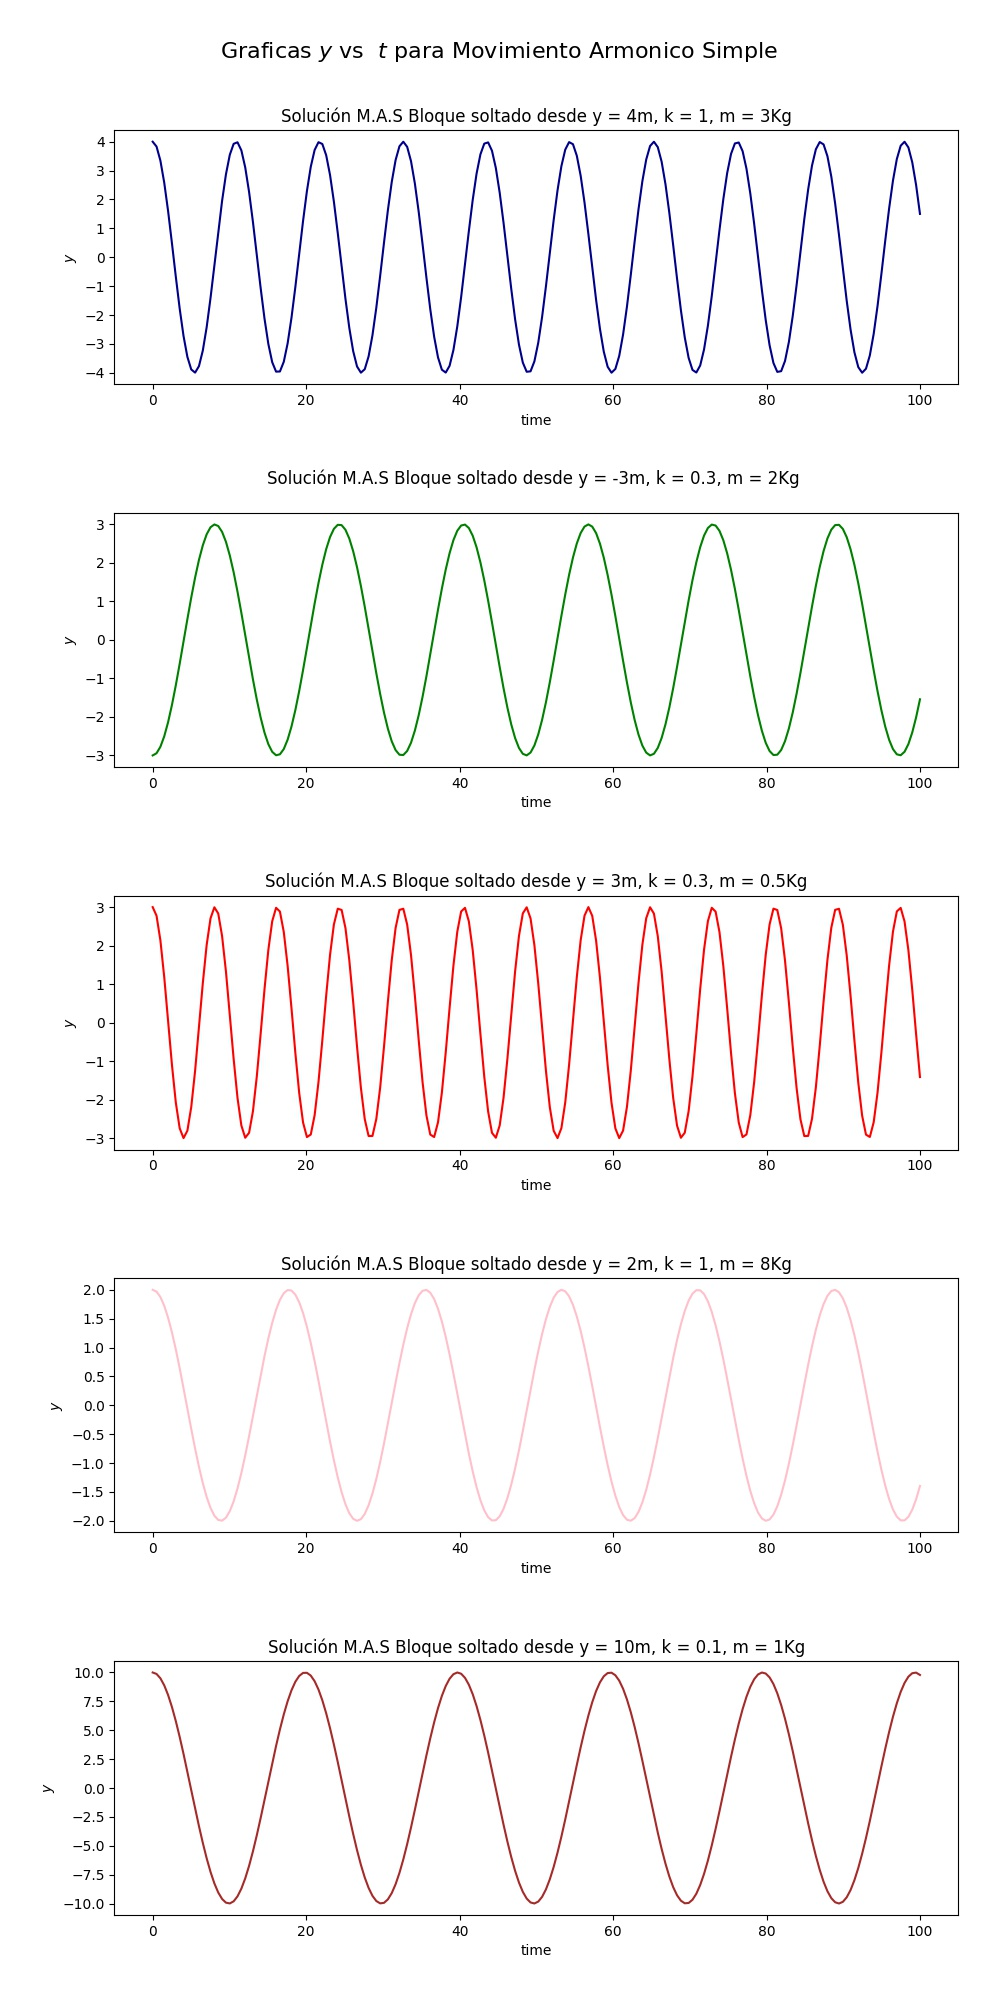
\includegraphics[width=0.8\textwidth]{MAS.jpg}
\caption{M.A.S}
\label{fig:Figura1}
\end{figure}

\subsection{Espacios de Fase}

Para hallar los espacios de fase graficamos $y'$ vs y.
Se tiene que la ecuación de la trayectoria es: $$\frac{y^2}{2E/k}+\frac{y'^2}{}2E/m=1$$ 

Donde podemos observar que estos caminos de fase representan una elipse, vemos que la energía se conserva para un sistema armónico simple como se puede ver en la Figura \ref{fig:Figura2}.

\begin{figure}
\centering
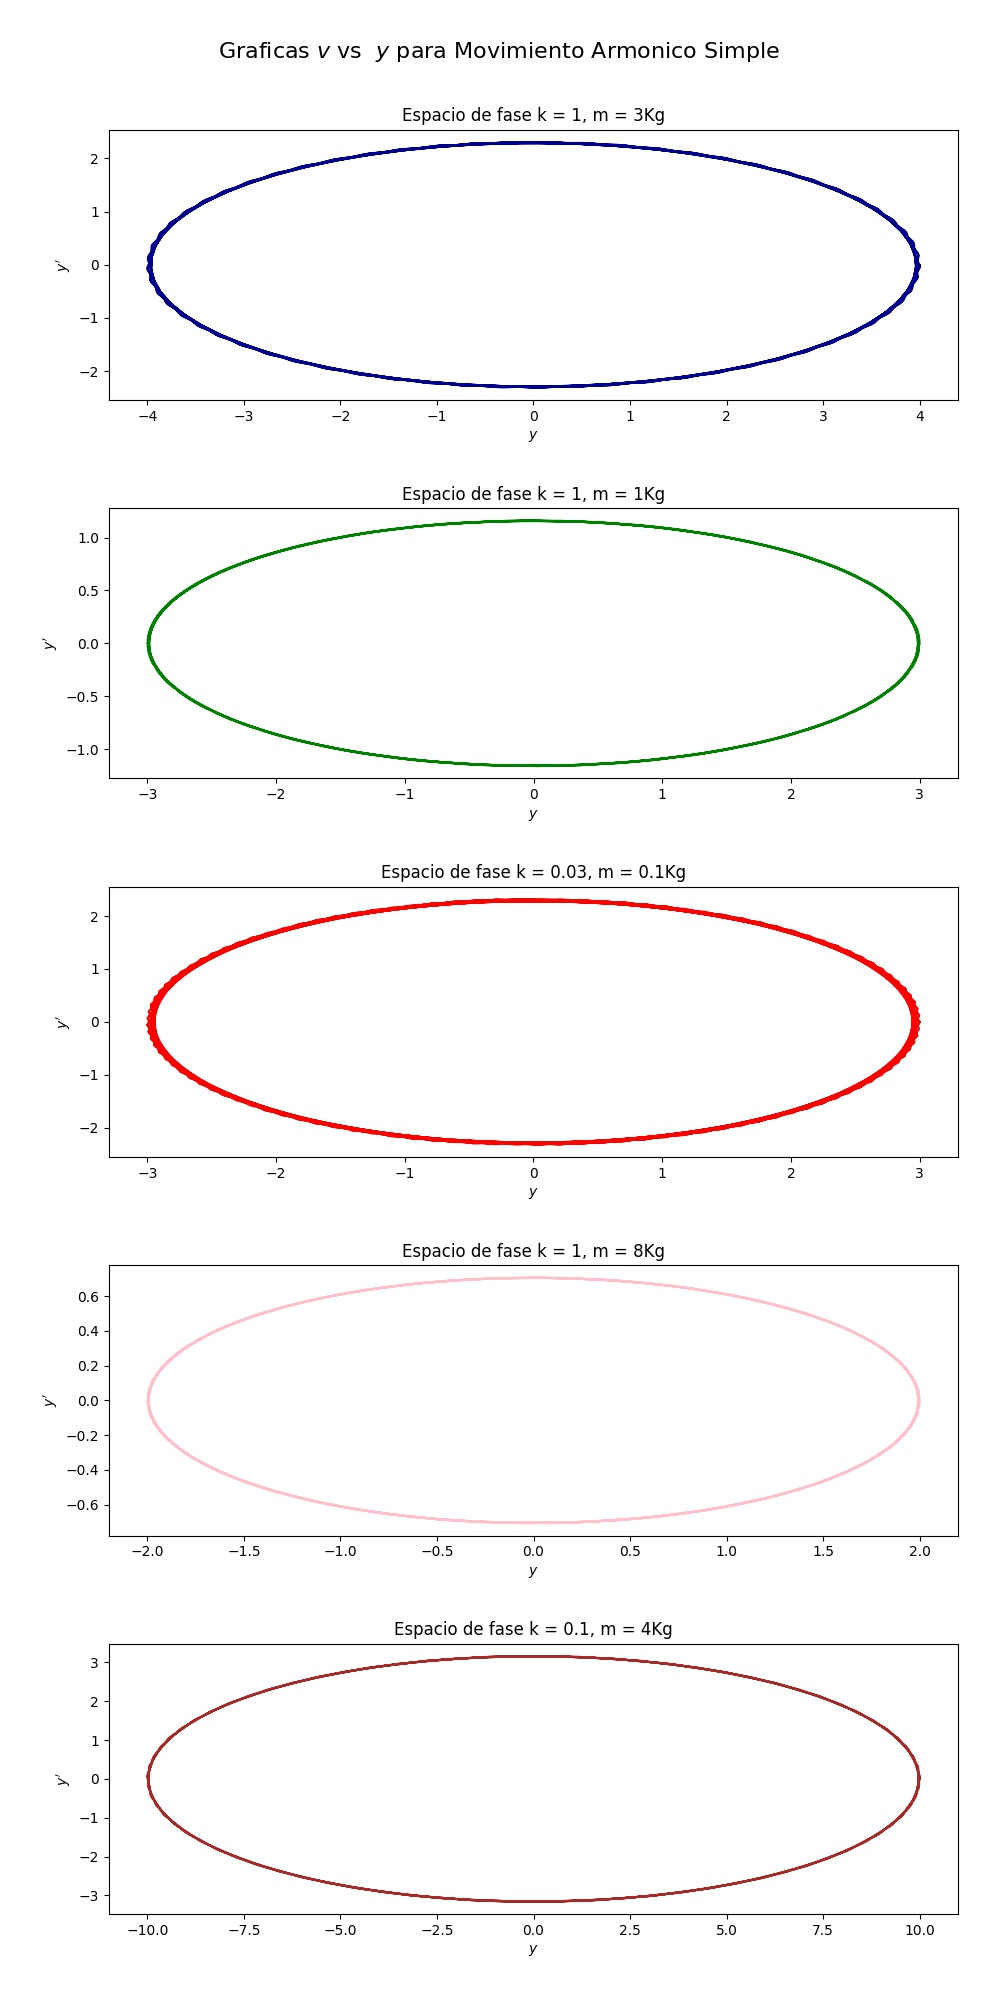
\includegraphics[width=0.8\textwidth]{MAS_FASE.jpg}
\caption{Espacios de fase de M.A.S}
\label{fig:Figura2}
\end{figure}


\section{Movimiento Armónico Amortiguado}

Para tratar el movimiento armónico amirtiguado, analizamos los mismos 5 casos solo que esta vez añadiendo el factor de amortiguamiento $\gamma$ para el sistema amortiguado, esto modifica las ecuaciones de movimiento lo cuál se ve traducido en los resultados obtenidos en la Figura \ref{fig:Figura3}.

Se toma el caso subamortiguado el cual se da para $\gamma < w_{0}$ y se observa que entre más grande sea el factor de amortiguamiento $\gamma$ el sistema oscilará menos y se frenará más rápido.

\begin{figure}
\centering
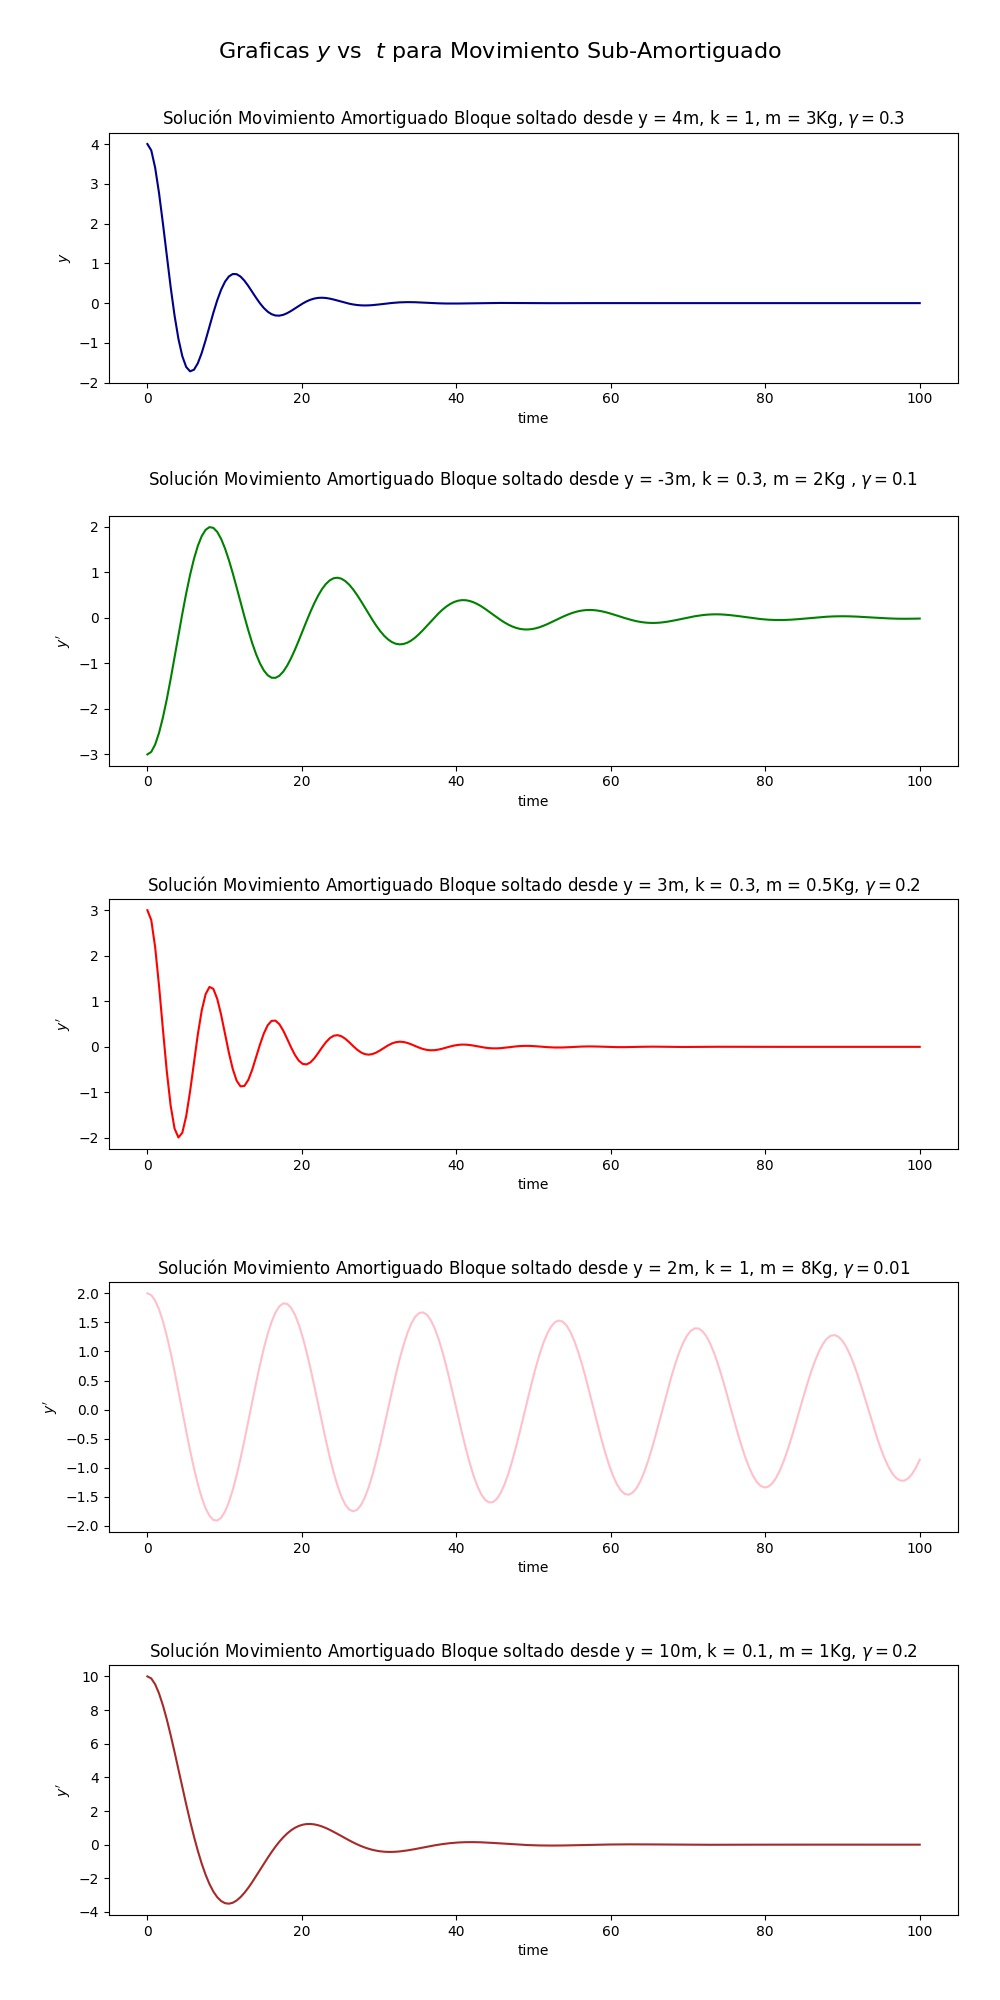
\includegraphics[width=0.8\textwidth]{Amortiguado.jpg}
\caption{Movimiento Amortiguado}
\label{fig:Figura3}
\end{figure}

\subsection{Espacios de Fase}

Podemos ver que la energía no se conserva, en los gráficos de $posición$ vs $tiempo$ se puede ver como el sistema se va quedando quieto, en el diagrama de fases presente en la Figura \ref{fig:Figura4}.

Al cambiar el problema a polares podemos ver que la trayectoria de fase es:  $\rho=wAe^{-\gamma t}$ lo cual representa una espiral, como lo son los resultados obtenidos en este caso.

\begin{figure}
\centering
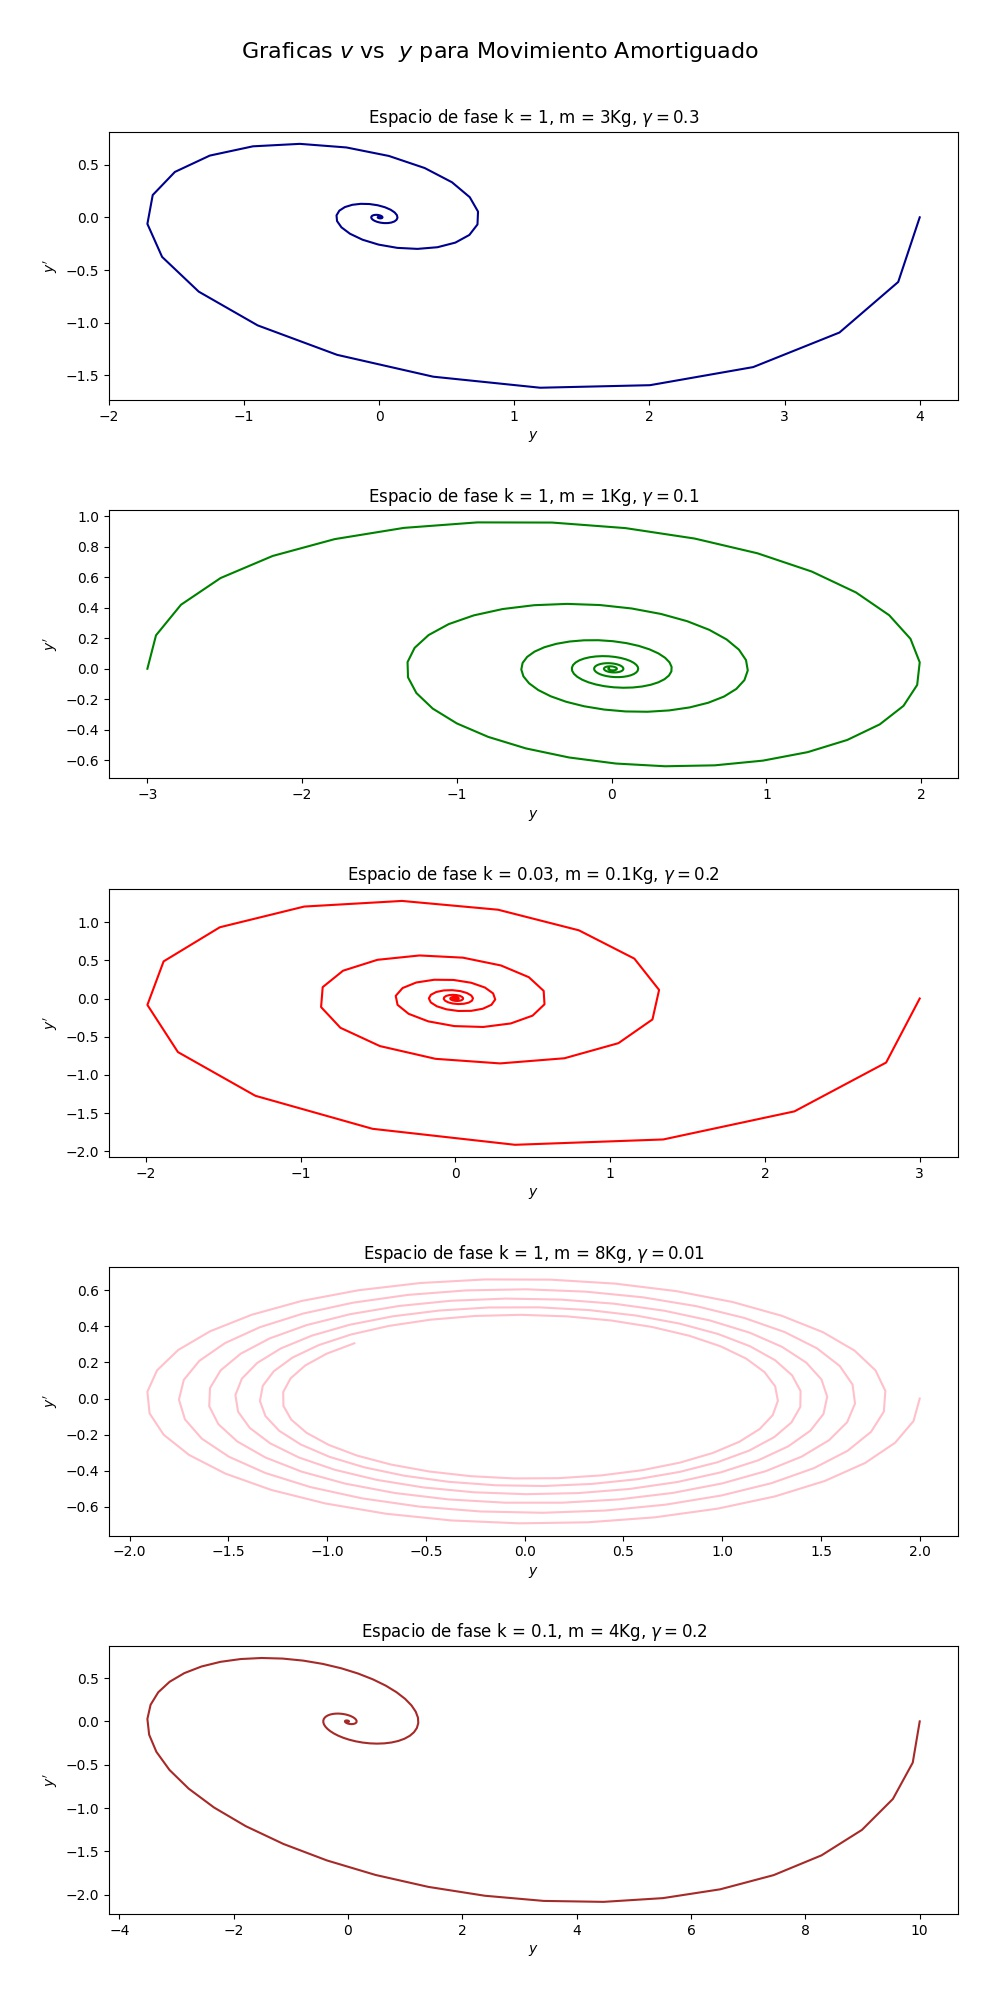
\includegraphics[width=0.8\textwidth]{Amortiguado_fases.jpg}
\caption{Espacios de Fase de Movimiento Amortiguado}
\label{fig:Figura4}
\end{figure}



















\end{document}